\subsection{Erdbebensicheres Bauen}

\begin{frame}
\frametitle{Historie und Spannungskarte}
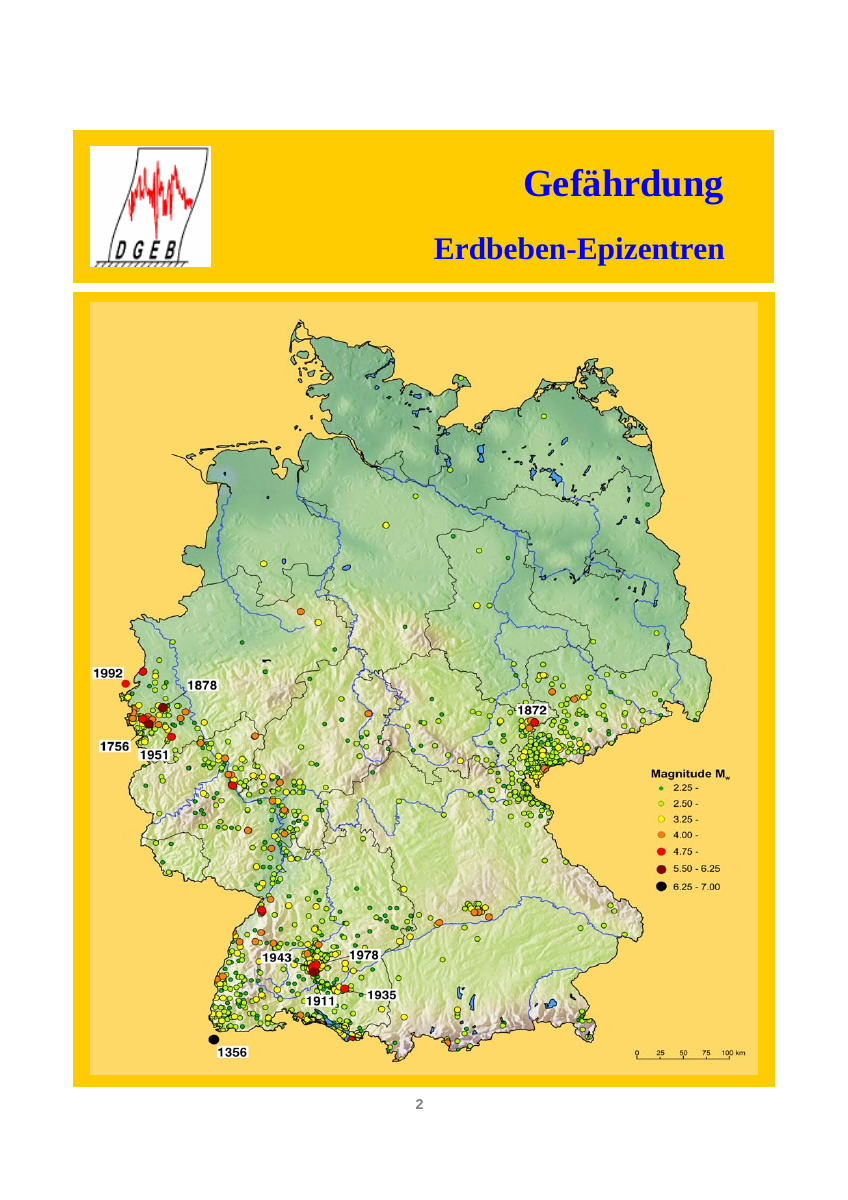
\includegraphics[width=0.43\textwidth]{fig_img/erdbeben_de} %TODO cite DGEB
\hfill
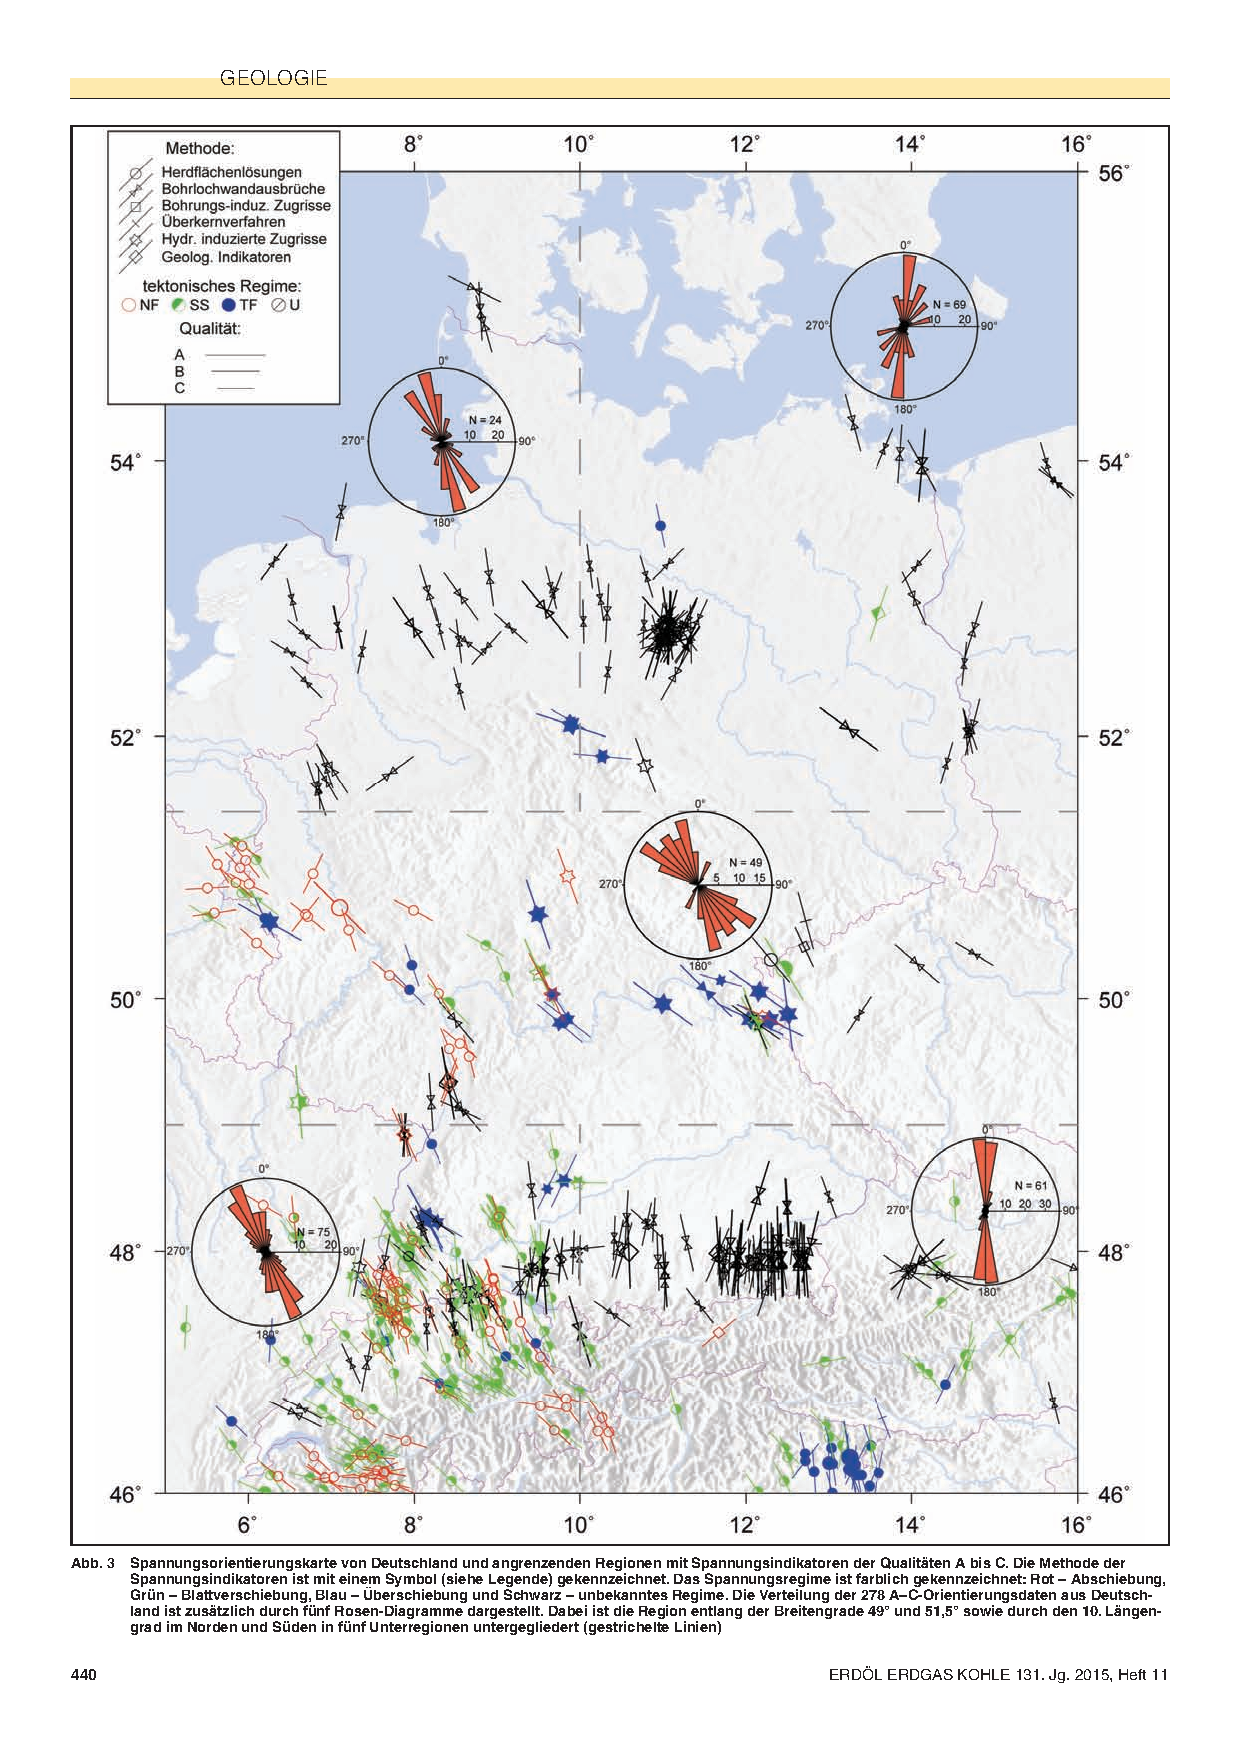
\includegraphics[width=0.4\textwidth]{fig_pdf/spannungslandkarte} %TODO stress map
\end{frame}


\begin{frame}
\frametitle{Effekte}
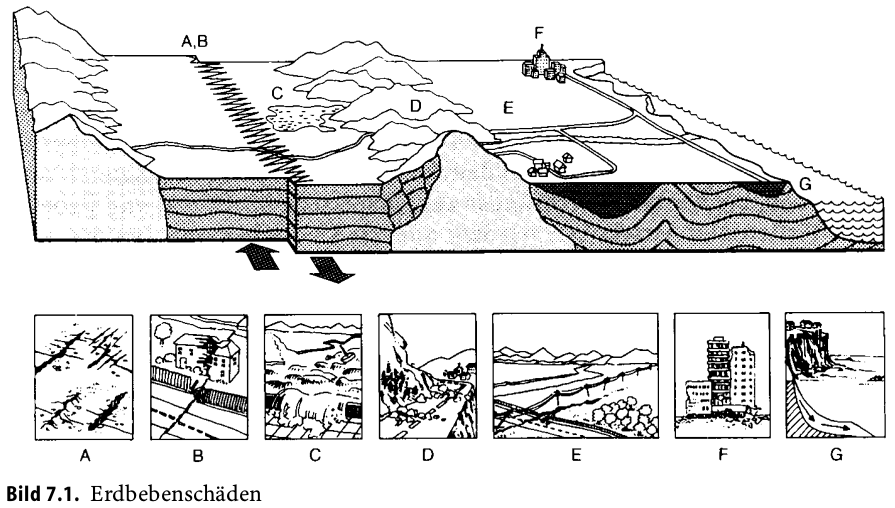
\includegraphics[width=0.95\textwidth]{fig_img/erdbebenschaeden} %TODO cite Studer
\end{frame}


\begin{frame}
\frametitle{Entstehung}
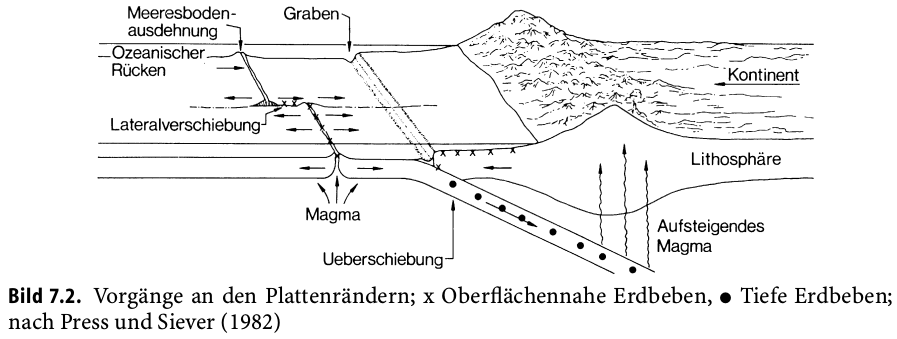
\includegraphics[width=\textwidth]{fig_img/plattenraender} %TODO cite Studer
\end{frame}


\begin{frame}
\frametitle{Verwerfungstypen}
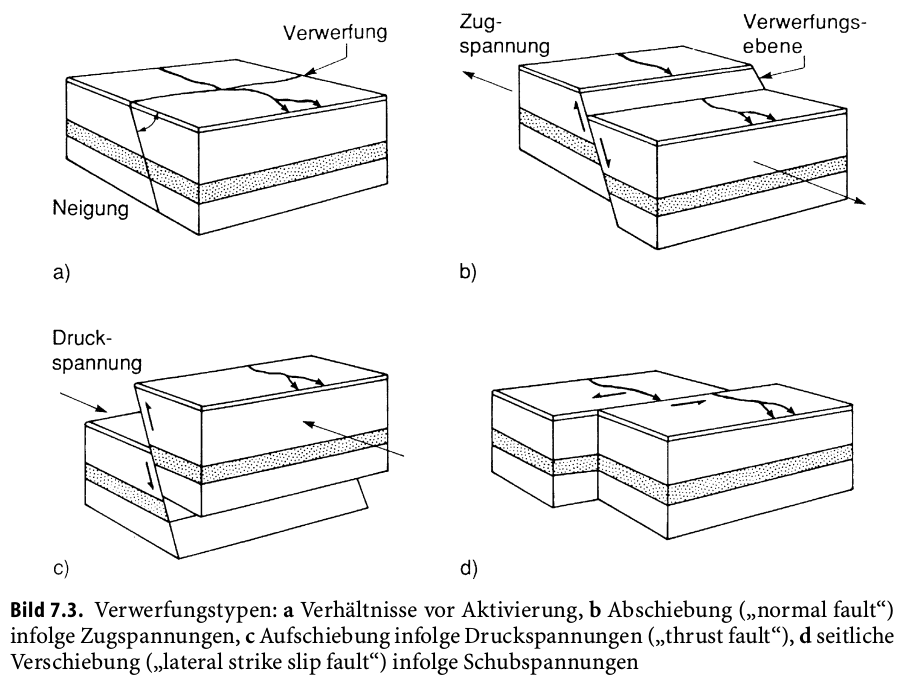
\includegraphics[width=0.72\textwidth]{fig_img/verwerfungstypen} %TODO cite Studer
\end{frame}


\begin{frame}
\frametitle{Geometrie}
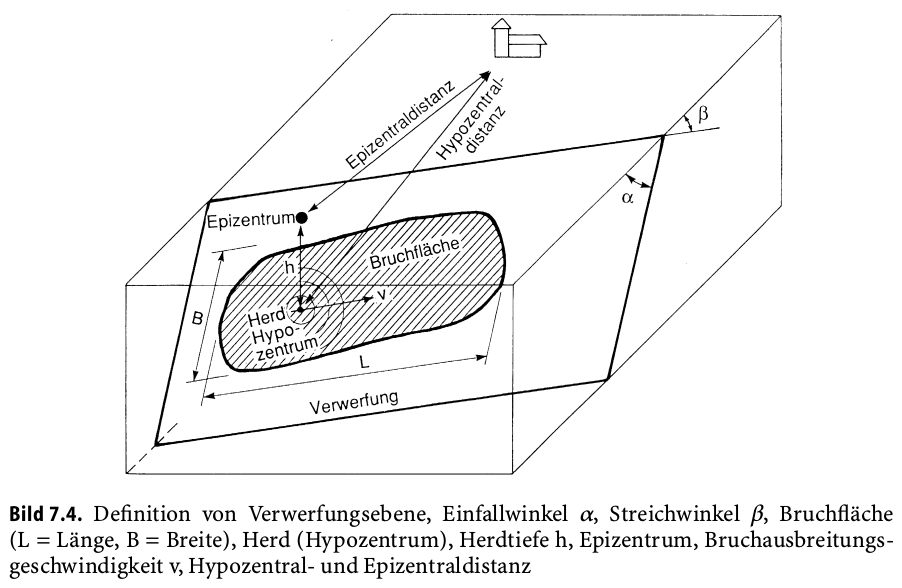
\includegraphics[width=0.83\textwidth]{fig_img/erdbebengeometrie} %TODO cite Studer
\end{frame}


\begin{frame}
\frametitle{Beschreibung}
\textbf{Intensität:} Phänomenologische Beschreibung nach hervorgerufener Wirkung\\
1 (nicht fühlbar) \dots 6 (Gebäudeschäden) \dots 12 (vollständig verwüstend) Klassifzierung nach EMS-1998

\bigskip

\textbf{Magnitude:} Maß für die freigesetzte Energie
\begin{itemize}
 \item Richter $M_\mathrm{L} = \log_{10}\left(\dfrac{\mathrm{max}(u_{\SI{100}{\kilo\metre}})}{u_\mathrm{ref}} \right)$ bezogen auf Referenzpunkt  % +1 entspricht Energie 31.6, Verschiebung 10 [Richter]
 \item Moment  $M_\mathrm{W}=\frac{2}{3}\log_{10}(M_0) - 6$  bezogen auf Erdbebenherd $M_0 = \mu A \Delta u$ $[M_0]=\SI{}{\newton\metre}$, mit Scherfestigkeit $\mu$ an der Bruchzone, Bruchfläche $A$ und mittlerer Verschiebung $\Delta u$  % [ToDo]
\end{itemize}
\end{frame}


\begin{frame}
\frametitle{Vorgehenskonzepte}
\begin{description}
 \item[deterministisch] sehr spezifisch (Ort, Szenario), modellbasiert (Quelle, Übertagungsmedium, Empfänger), Problem Parameterbestimmung
 
 \item[probabilistisch] ausgehend von bisherigen räumlichen und zeitlichen Verläufen werden erdenkliche Erdbeben mit Wahrscheinlichkeiten versehen.
\end{description}

\vfill

Bewertung hinsichtlich
\begin{itemize}
 \item Baugrunderschütterung
 \item Bodenverflüssigung
 \item Hangrutschungen
 \item Risse an der Erdoberfläche
\end{itemize}


\end{frame}


\begin{frame}
\frametitle{Berücksichtigung in der Auslegung}
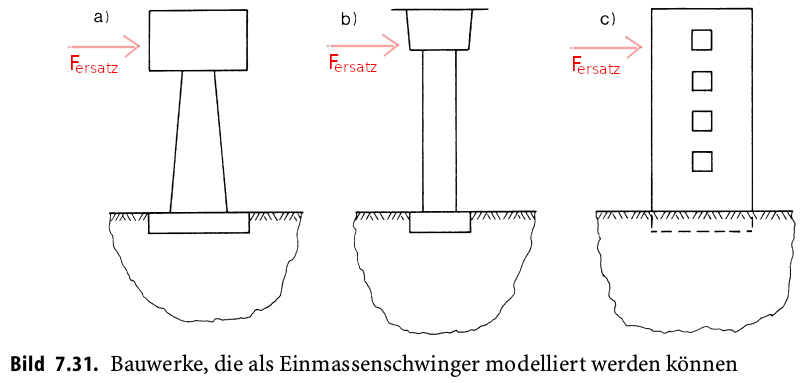
\includegraphics[width=\textwidth]{fig_img/einmassenmodell_erdbeben}

%Idee: Bauwerke (oder einzelne Schwingformen) lassen sich durch Einmassenschwinger annähern
\end{frame}


\begin{frame}
\frametitle{Antwortspektrum}  % allgemein/standortspezifisch
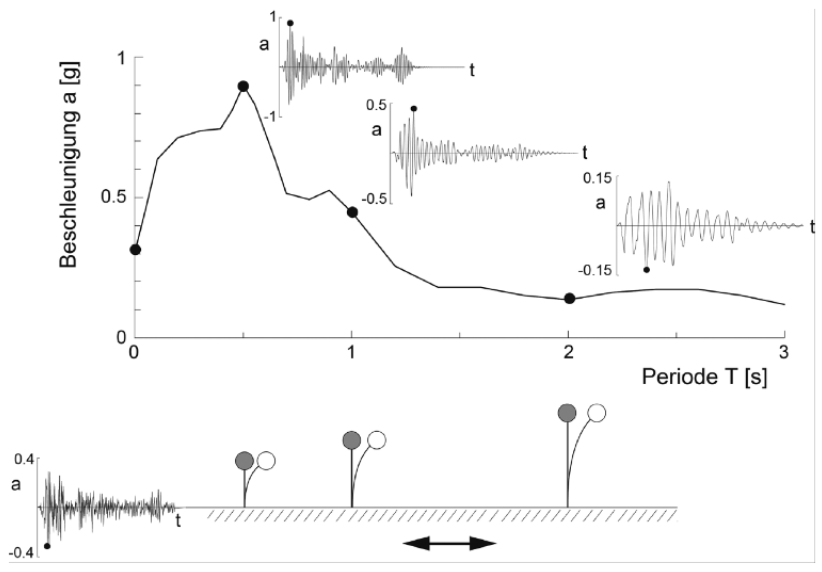
\includegraphics[width=0.77\textwidth]{fig_img/antwortspektrum} %TODO cite Vrettos
\end{frame}


\begin{frame}
\frametitle{Bemessungsspektrum}  % allgemein/standortspezifisch
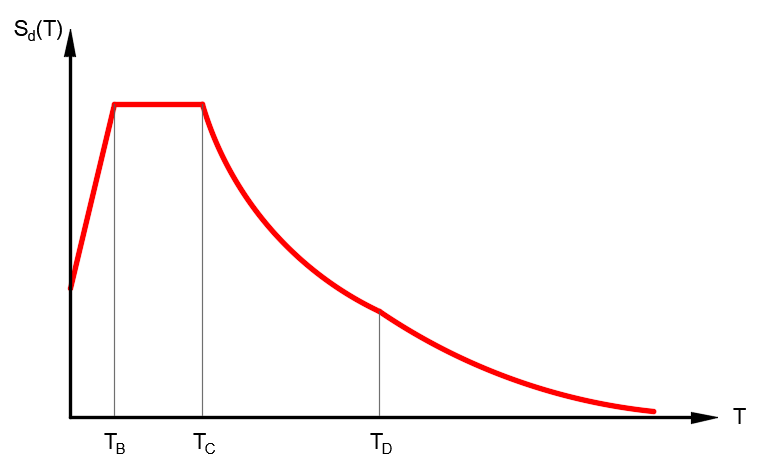
\includegraphics[width=0.75\textwidth]{fig_img/bemessungsspektrum} %TODO cite

Das Bemessungsspektrum ist ein ``geglättetes'' und ``informationsangereichertes'' Antwortspektrum. 
\end{frame}

\begin{frame}
\frametitle{Auslegung {\normalsize anhand des Bemessungspektrums}}  % allgemein/standortspezifisch 
\only<1>{
\begin{align*}
0<T\le T_\mathrm{B}  &: \quad S_\mathrm{d}(T)=a_\mathrm{gR} \gamma_l S \left[ 1+\frac{T}{T_\mathrm{B}}\left(\frac{2.5}{q}-1\right) \right] \\
T_\mathrm{B}<T\le T_\mathrm{C}  &: \quad S_\mathrm{d}(T)=a_\mathrm{gR} \gamma_l S \frac{2.5}{q}\\
T_\mathrm{C}<T\le T_\mathrm{D}  &: \quad S_\mathrm{d}(T)=a_\mathrm{gR} \gamma_l S \frac{2.5}{q}\frac{T_\mathrm{C}}{T}\\
T_\mathrm{D}<T\le \SI{4}{\second}  &: \quad S_\mathrm{d}(T)=a_\mathrm{gR} \gamma_l S \frac{2.5}{q}\frac{T_\mathrm{C} T_\mathrm{D}}{T^2}
\end{align*}
$T$ ist die Periodendauer des Einmassenschwingers, alle übrigen Parameter charakterisieren das Erdbebengebiet, den Baugrund und das Bauwerk.
}%only

\only<2>{
$S_\mathrm{d}$ entspricht einer Beschleunigung, demzufolge berechnet sich die Ersatzkraft
\begin{equation*}
 F_\mathrm{ersatz} = S_d(T) m \lambda,
\end{equation*}
wobei $\lambda$ ein Korrekturwert für die Stockwerke ist.

\vfill

Die Periode eines Gebäudes kann in Abhängigkeit der Höhe $h$ geschätzt werden
\begin{equation*}
 T = C_t h^{3/4}
\end{equation*}
wobei $C_t$ das Tragwerk charakterisiert ($C_t=\SI{0.085}{}$ für biegesteife räumliche Stahlrahmen, $C_t=\SI{0.075}{}$ für biegesteife räumliche Stahlbetonrahmen und $C_t=\SI{0.050}{}$ für andere Rahmen).

}%


\end{frame}




\begin{frame}
\frametitle{Konstruktionshinweise}  % allgemein/standortspezifisch
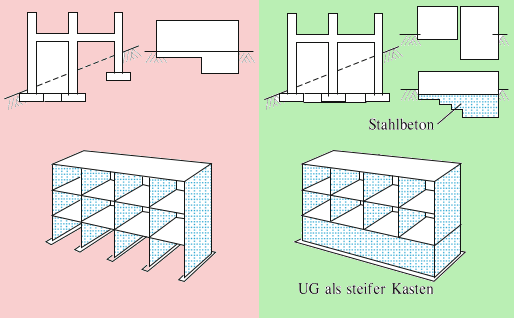
\includegraphics[width=0.495\textwidth]{fig_img/erdbebensicher_konstruieren1} 
\hfill
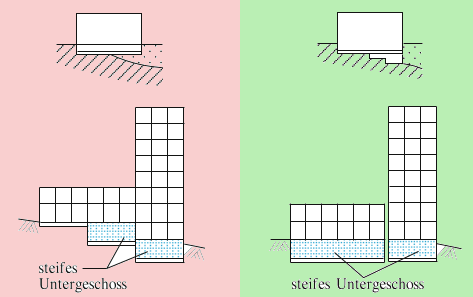
\includegraphics[width=0.495\textwidth]{fig_img/erdbebensicher_konstruieren2} 
\cite{Schmidt2017}
\end{frame}
